w%Esta charla puede ser descargada en http://people.ubuntu.com/~naguilarg/charlas/Debian-Edu
%Autor: Norman GArcía Aguilar norman@risuep.net

\documentclass{beamer}
%\usepackage[latin1]{inputenc}
\usepackage[spanish]{babel}
\usepackage{graphicx}
\usetheme{Warsaw}
\title{Escuelas libres con Debian Edu}
\author[n0rman]{Norman Garc\'ia \\ \texttt{norman@riseup.net}}
\institute{Debian Nicaragua}
\date{Mayo 24, 2012}
\begin{document}

\begin{frame}
	\titlepage
\end{frame}

\begin{frame}{Contenido}
	\tableofcontents
\end{frame}


\section{Introducci\'on}

\begin{frame}
\frametitle{¿Qu\'e es Debian Edu?}
        
	\begin{itemize}
                \pause \item Debian Edu es un derivado de la distribuci\'on Debian GNU/Linux.
		\pause \item Una variante de Debian para escuelas.
		\pause \item Que pre-configura un ambiente de red educativo.
		\pause \item Puede ser usado fuera del \'ambito educativo.
		\pause \item Tambi\'en conocido como Skolelinux.
       \end{itemize}

\end{frame}

\begin{frame}
\frametitle{Metas de Debian Edu}    
        \begin{itemize}
                \pause \item Proveer una soluci\'on educativa basada 
			en Software Libre.
		\pause \item Clasificar y empaquetar Software Libre
			orientado a educaci\'on.
		\pause \item Escribir documentaci\'on para el manejo 
			de apicaciones para educaci\'on.
		\pause \item Ser conocido internacionalmente, traducido
			a muchos idiomas.
        \end{itemize}
\end{frame}

\section{M\'as sobre Debian Edu}
\begin{frame}
\frametitle{Requisitos}
\begin{itemize}
	\pause \item Computadoras con  i386, amd64 o powerpc.
	\pause \item Dos tarjetas de red para servidor.
	\pause \item Al menos 2Gb RAM para 30 clientes, y 4GB para 50-60 clientes.
	\pause \item Almacenamiento variable, 15 Gb para una estaci\'on de 
		trabajo, 20 Gb para un servidor de clientes ligeros y al 
		menos 30 Gb para el servidor principal.
	\pause \item Los clientes ligeros pueden funcionar con 64 MB de RAM y 
		133 MHZ de procesador, aunque se recomienda 128 MB de RAM y 
		procesadores de mayor velocidad.
	\pause \item Para estaciones de trabajo se recomienda 256 Mb de RAM.

\end{itemize}
\end{frame}

\begin{frame}
\frametitle{¿Por qu\'e Debian Edu?}
    \begin{itemize}
             \pause \item Debian Free Software Guidelines (DFSG).
	     \pause \item Contrato social de Debian.
	     \pause \item Pol\'iticas de Debian.
	     \pause \item Calidad y Libertad.
    \end{itemize}
\end{frame}

\begin{frame}
\frametitle{¿Por qu\'e Debian Edu?}
       \begin{itemize}
                \pause \item Sistema out-of-the-box con LDAP, Kerberos, NFS, Samba, DNS, DHCP, CUPS, nagios, munin.
                \pause \item LDAP GUI Gosa.
                \pause \item Entorno de escritorio KDE4 por defecto, pero tambi\'en se soporta LXDE y Gnome.
		\pause \item Instalaci\'on PXE.
		\pause \item Buena documentaci\'on. (Necesitamos ayuda en traducci\'on a Espanol).
        \end{itemize}
\end{frame}

\begin{frame}
\frametitle{Eventos}
        \begin{center}
                 
\includegraphics[scale=0.50]{../img/debconf_12_nicaragua.png}
        \end{center}
\end{frame}

\begin{frame}
	\begin{center}
		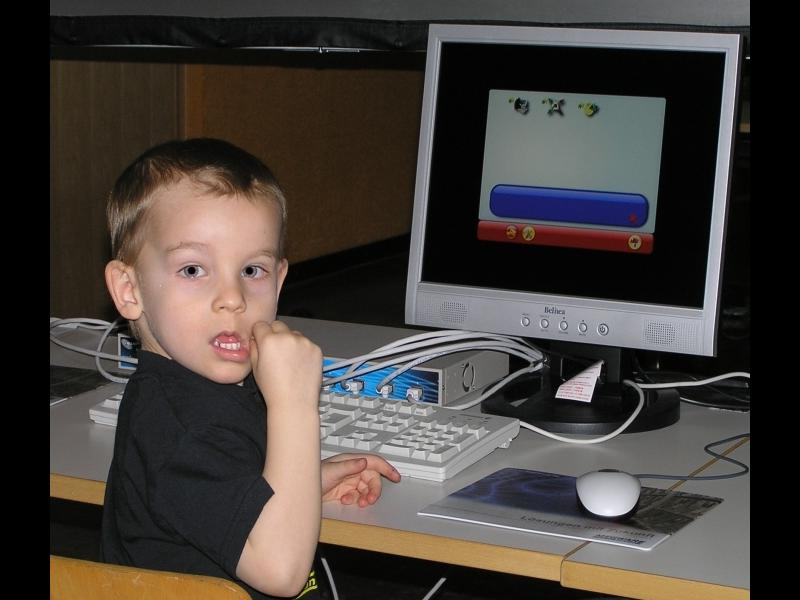
\includegraphics[scale=0.30]{../img/ninoedu.jpg}
	\end{center}
\end{frame}

\section{Razones para contribuir}

\begin{frame}
\frametitle{¿Qu\'e gano?}
             \begin{enumerate}
		\pause \item Aumentar mis conocimientos.
		\pause \item Convertirme en Debian Developer.
		\begin {itemize}
			\pause \item Derecho de voto.
			\pause \item Poder incorporar o hacer mejoras de cualquier software al sistema operativo Debian GNU/Linux.
			\pause \item Acceso a recursos del proyecto como servidores.
			\pause \item Tomar decisiones propias sobre su propio trabajo dentro del proyecto.
			\pause \item Postularse como Debian Project Leader.
			\pause \item \alert{NO ES NECESARIO MANTENER PAQUETES.}
		\end{itemize}
		\pause \item algunos DD que no mantienen paquetes.
		\begin{itemize}
			\pause \item Martin Baggage \texttt{brother-}: Mantiene traducciones a Sueco.
			\pause \item Francesa Ciceri \texttt{MadameZou}: Mantiene traducciones a Italiano, el sitio web y apoya al equipo de publicidad.
			\pause \item Matt Zimmerman: Se encarga de relaciones con distribuciones derivadas de Debian.
		\end{itemize}
	     \end{enumerate}
\end{frame}

\begin{frame}
\frametitle{¿Qu\'e gano?}
	\begin{center}
                 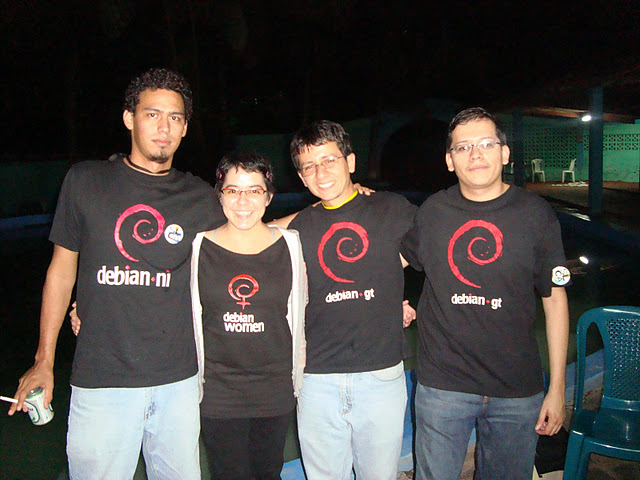
\includegraphics[scale=0.30]{../img/DSC03610.JPG}
	\end{center}
\end{frame}


\begin{frame}
\frametitle{¿Qu\'e gano?}
	\begin{center}
                 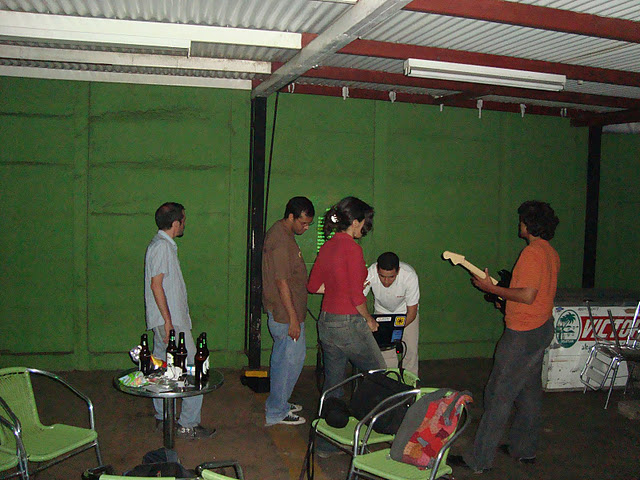
\includegraphics[scale=0.30]{../img/dsc04738.jpg}
	\end{center}
\end{frame}


\begin{frame} 
\frametitle{¿Qu\'e gano?}
                 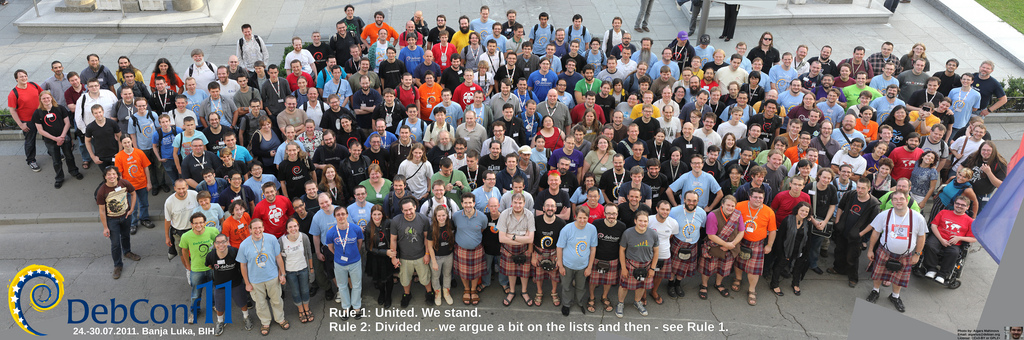
\includegraphics[scale=0.30]{../img/dc11photogroup.jpg}
\end{frame}


\section{Gracias}


\begin{frame}
\frametitle{FIN}
	\begin{enumerate}
		\pause \item Presentaci\'on: Escuelas libres con Debian Edu.
		\pause \item Presentaci\'on basada en
			\begin{itemize}
				\pause \item Debian Edu por \texttt{Holger Levsen}
%					Puede descargar en  https://penta.debconf.org/penta/file/event_attachment/177?filename=howto-contribute.pdf
			\end{itemize}
		\pause \item Presentado por: Norman Garc\'ia  \texttt{norman@riseup.net}
		\pause \item Mayo 24, 2012
		\pause \item Licencia: Creative Commons Atribuci\'on-CompartirIgual 3.0 Unported (CC BY-SA 3.0)
	\end{enumerate}

	\begin{center}
  		 
\includegraphics[scale=0.20]{../img/cclogo.png}
	\end{center}

\end{frame}
\end{document}
